\documentclass[11pt]{article}
\usepackage{geometry}
\usepackage{tocbibind}
\usepackage{pslatex}
\usepackage{url}
\usepackage{multicol}
\usepackage{array}

%Check if we are compiling under latex or pdflatex
\ifx\pdftexversion\undefined
	\usepackage[dvips]{graphicx}
	\geometry{verbase,letterpaper,margin=1.0in,nohead}
	\usepackage[ps2pdf,colorlinks,bookmarks=true]{hyperref}
\else
	\usepackage[pdftex]{graphicx}
	\geometry{verbose,letterpaper,margin=1.0in,nohead,pdftex}
	\usepackage[pdftex,colorlinks,bookmarks=true,bookmarksopen=true,pdfpagemode=node]{hyperref}
\fi

	

\begin{document}
	
\pagestyle{plain}

\begin{titlepage}			%Title cover
\begin{center}

\vspace*{1in}
\Large
\textsf{\href{http://www.cybermation.com}{Cybermation} \& \href{http://www.ece.toronto.edu}{University of Toronto} \ Middleware Systems Research Group} \\
\vfill
\LARGE
\textsf{\textbf{Federated Publish/Subscribe Middleware Project}} \\
\bigskip
\huge
\textbf{Database Binding Design Document}

\vfill \vfill

\large

\href{mailto:wan_pengcheng@yahoo.com}{Pengcheng Wan} \\
\bigskip
\href{mailto:acheung@cybermation.com, e.fidler@utoronto.ca,
jacobsen@eecg.utoronto.ca, david.matheson@utoronto.ca,
smankovski@cybermation.com, pwan@cybermation.com}{group email}

\vfill

\textbf{Toronto, Ontario} \\
\bigskip
Last Updated: \today \\
Last Update By: Pengcheng Wan

\end{center}
\end{titlepage}				%Tile Cover

\normalsize
\newpage

\tableofcontents
\newpage

\setlength{\parindent}{0mm}
\setlength{\topsep}{0mm}
\setlength{\partopsep}{0mm}

%The start of the text
\section{Database Binding}
A publish/subscribe system is a middleware communication service that delivers
messages from a sender to one or more receivers using the preferences expressed
by those receivers, rather than relying on an explicit destination address set
by the sender. Database Binding in the project is to specify how the outer database 
can map and implement the publish and subscribe functionality in the system.

\subsection{The Choice of Database}    %The first part
The choice of database software for Java applications in this system is critical. Basically, we focus the choice of databases on the open source databases which are under the GNU General Public Licence(GPL). We choose two major open source databases MySQL 4.0.13 and PostgreSQL 7.3.4 as our comparision.
\subsubsection{MySQL 4.0.13}
MySQL product is one of the world's most popular open source database. Its architecture makes it extremely fast and easy to customize.
\begin{itemize}
\item Advance Feature\\
MySQL is the fastest full-featured SQL engine around, requires the least overall hardware and platform resources to operate in production. MySQL ships with a high-capacity engine, which can support tens of millions of records and hundreds of concurrent users. The other feature of MySQL is that it can run the database in a production Windows 2000/XP environment.

\item Limitation
\begin{enumerate}
\item \emph{MySQL has no subqueries}\\
Instead of performing one complex query that is entirely processed on the database end, MySQL users have to perform two or more serial queries that each must go over inter-process or network communicatoin between the app and the database. This significantly reduces the speed advantafes of MySQL. This feature include nested SELECT queries will be supported in version 4.1.
\item \emph{MySQL has no stored procedures}\\
If a series of DB actiontions need to be performed in a block, MySQL requires each SQL statement to be sent from the app, again in a serial manner, again over IPC or network. Support for stored procedures will be introduced in version 5.0.
\item \emph{MySQL has no triggers or foreign key constraints}\\
Data invariants must be maintained by application-level code, which requires building carefully-planned abstractions to guarantee integrity(for every means of accessing your Database), and even more unnecessary back-and-forth communication between the app and the database. By using the InnoDB or Berleley DB(BDB) storage engines not the standard MySQL storage engine, the MySQL database server supports transaction and foreign key constraints. Support for this feature in the standard MySQL storage engine will be included in version 5.0. 
\item \emph{MySQL only has table-level locking}\\
Only one user can write to a table at the same time. If one need row-level locking, she or he needs to use the InnoDB storage engine.
\item \emph{MySQl does not support view}\\
Views allow developer to configure alternative views of existing tables without changing the underlying table structure. They can be used to grant limited access to tables, or make it easier to construct certaim types of queries. Views are scheculed to be supported in version 5.1.
\end{enumerate}

\end{itemize}

\subsubsection{PostgreSQL 7.3.4}
PostgreSQL is widely considered the most advanced open source database in the world. It provides a wealth of features that are usually only found in commercial databases such as DB2 or Oracle. 

\begin{itemize}
\item Advance Feature
\begin{enumerate}
\item \emph{Object-relational DBMS}\\
PostgreSQL is capable of handling complex objects and rules. Examples of the functionality that PostgreSQL supports are declarative queries in SQL, concurrency control, transactions, query optimization, and multiuser support.
\item \emph{Highly extensible}\\
PostgreSQL supports user-defined operators, functions, access methods, and data types.
\item \emph{Comprehensive SQL support}\\
PostgreSQL supports the core SQL99 specification and includes advanced features such as SQL92 joins, inheritance, and arrays.
\item \emph{Referential integrity}\\
PostgreSQL supports referential integrity, which is used to insure the validity of a database's data.
\item \emph{Flexible API}\\
PostgreSQL includes an extensive API. The flexibility of the PostgreSQL API has allowed vendors to provide development support easily for the PostgreSQL database. PostgreSQL arguably has the largest amount of interface capabilities of any database. These interfaces include Object Pascal, Python, Perl, PHP, ODBC, Java/JDBC, Ruby, TCL, C/C++, and Pike.
\item \emph{Procedural languages}\\
PostgreSQL has support for internal procedural languages, including a native language called PL/pgSQL. The language is comparable to the Oracle procedural language, PL/SQL. Another real advantage to PostgreSQL is its ability to use Perl, Python, or TCL as an embedded procedural language.
\end {enumerate}
\item Limitation\\
The main disadvantages with PostgreSQL appear to be a maximum row size limit of 8K, a limit on connections to 32 and the rather less than inviting commands e.g. lack of delete column command, no view/describe table and so on. Also PostgreSQL is still a little bit slower than MySQL now and can not run directly in windows platform.
\end{itemize}
\subsubsection{Conclusion}
In summary, both databases are pretty good. They are both free and extremely fast in comparison to some desktop databases. Both are supported by an active developer community. Considering our database design scheme, we need the database to support \emph{subselect, view, transction} and other nifty features, so we choose PostgreSQL as our database.


\subsection{Major Cases}   %The second part
The major cases include Attaching a Database, Historical Query. The detail explanation is in the architecture document.

\subsection{Database Design Scheme}  %The third part
The events are stored in the historical database using the following eight (sets
of) tables. The stored events are: \texttt{stock(volume=100, code=`CYB')} and
\texttt{stock(price=798.23, code=`CYB')}.

\begin{table}[!h]					%Events table
\centering
\begin{tabular}{c|c|c|c|c|c|c}
\textbf{EventID} & ClassID & DataID & LastHopID & PayLoad & Priority & Time \\
\hline
1 & 1 & 1 & 128.168.23.90 & $<$null$>$ & 3 & $<$time$>$ \\
2 & 1 & 2 & 128.168.23.90 & $<$null$>$ & 2 & $<$time$>$
\end{tabular}
\caption{EVENTS table}
\end{table}

\begin{table}[!h]					%EventData table and Classes table
\begin{minipage}[!h]{0.5\linewidth}
\centering
\begin{tabular}{c|c}
\textbf{DataID} & \textbf{PairID} \\
\hline
1 & 1 \\
1 & 2 \\
2 & 3 \\
2 & 2
\end{tabular}
\caption{EVENTDATA table}
\end{minipage}
\begin{minipage}[!h]{0.5\linewidth}
\centering
\begin{tabular}{c|c}
\textbf{ClassID} & ClassName \\
\hline
1 & stock
\end{tabular}
\caption{CLASSES table}
\end{minipage}
\end{table}

\begin{table}[!h]					%Pairs table
\centering
\begin{tabular}{c|c|c|c|c}
\textbf{PairID} & AttributeID & LongValueID & DoubleValueID & StringValueID\\
\hline
1 & 1 & 1 & $<$null$>$ & $<$null$>$\\
2 & 3 & $<$null$>$ & $<$null$>$ & 3\\
3 & 2 & $<$null$>$ & 2 & $<$null$>$\\
\end{tabular}
\caption{PAIRS table}
\end{table}

\begin{table}[!h]						%Attributes table and LongValues table
\begin{minipage}[!h]{0.5\linewidth}
\centering
\begin{tabular}{c|c|c}
\textbf{AttributeID} & AttributeName & AttributeType \\
\hline
1 & volume & INTEGER \\
2 & price & DOUBLE \\
3 & code & STRING \\
\end{tabular}
\caption{ATTRIBUTES table}
\end{minipage}
\begin{minipage}[!h]{0.5\linewidth}
\centering
\begin{tabular}{c|c}
\textbf{ValueID} & LongValue \\
\hline
1 & 100 \\
\end{tabular}
\caption{LONGVALUES table}
\end{minipage}
\end{table}

\begin{table}[!h]							%DoubleValues table and StringValues table
\begin{minipage}[!h]{0.5\linewidth}
\centering
\begin{tabular}{c|c}
\textbf{ValueID} & DoubleValue \\
\hline
2 & 798.23 \\
\end{tabular}
\caption{DOUBLEVALUES table}
\end{minipage}
\begin{minipage}[!h]{0.5\linewidth}
\centering
\begin{tabular}{c|c}
\textbf{ValueID} & StringValue \\
\hline
3 & `CYB'
\end{tabular}
\caption{STRINGVALUES table}
\end{minipage}
\end{table}

The above tables will be created through a sql script file \verb+create_table.sql+ and at the same time we will create a messages view for these tables in this script file.
\begin{itemize}
\item Create Tables \\
- Table structure for table 'CLASSES'\\
CREATE TABLE classes (\\
\verb+    +Class\_ID serial,      \\  
\verb+    +Class\_Name varchar(64) NOT NULL,\\
\verb+    +PRIMARY KEY (Class\_ID)\\
);\\

- Table structure for table 'ATTRIBUTES'\\
CREATE TABLE attributes (\\
\verb+    +Attribute\_ID serial,          \\        
\verb+    +Attribute\_Name varchar(64) NOT NULL ,\\
\verb+    +Attribute\_Type char(6) NOT NULL,  \\  
\verb+    +PRIMARY KEY  (Attribute\_ID)\\
);\\

- Table structure for table 'INTEGERVALUES'\\
CREATE TABLE longvalues (\\
\verb+    +Value\_ID serial,				\\		     
\verb+    +Long\_Value integer NOT NULL,\\
\verb+    +PRIMARY KEY  (Value\_ID)\\
);\\

- Table structure for table 'DOUBLEVALUES'\\
CREATE TABLE doublevalues (\\
\verb+    +Value\_ID serial,	 			\\		
\verb+    +Double\_Value float NOT NULL,\\
\verb+    +PRIMARY KEY  (Value\_ID)\\
);\\

- Table structure for table 'STRINGVALUES'\\
CREATE TABLE stringvalues (\\
\verb+    +Value\_ID serial,				\\		
\verb+    +String\_Value char(20)   NOT NULL,\\
\verb+    +PRIMARY KEY  (Value\_ID)\\
);\\

- Table structure for table 'PAIRS'\\
CREATE TABLE pairs (\\
\verb+    +  Pair\_ID integer NOT NULL,\\
\verb+    +  Attribute\_ID integer NOT NULL,\\
\verb+    +  Long\_ValueID integer,\\
\verb+    +  Double\_ValueID integer,\\
\verb+    +  String\_ValueID integer,\\
\verb+    +  PRIMARY KEY (Pair\_ID),\\
\verb+    +  FOREIGN KEY (Attribute\_ID) REFERENCES attributes (Attribute\_ID) ON DELETE SET NULL\\
);\\

- Table structure for table 'EVENTDATA'\\
CREATE TABLE eventdata (\\
\verb+    +  Data\_ID integer NOT NULL,\\
\verb+    +  Pair\_ID integer NOT NULL,\\
\verb+    +  PRIMARY KEY (Data\_ID, Pair\_ID),\\
\verb+    +  FOREIGN KEY (Pair\_ID) REFERENCES pairs (Pair\_ID) ON DELETE SET NULL\\
);\\

- Table structure for table 'EVENTS'\\
CREATE TABLE events (\\
\verb+    +  Event\_ID varchar(16) NOT NULL,\\
\verb+    +  Class\_ID integer NOT NULL,\\
\verb+    +  Data\_ID integer  NOT NULL,\\
\verb+    +  LastHop\_ID varchar(30) NOT NULL,\\
\verb+    +  Payload bytea,	\\
\verb+    +  Priority smallint NOT NULL,\\
\verb+    +  Time timestamp(6) NOT NULL,\\
\verb+    +  PRIMARY KEY (Event\_ID),\\
\verb+    +  FOREIGN KEY (Class\_ID) REFERENCES classes (Class\_ID) ON DELETE SET NULL\\
);\\
\item Create Views \\
The view of messages should be like this: \\
\begin{table}[!h]					%Messages table
\centering
\begin{tabular}{c|c|c|c|c|c|c}
\textbf{EventID} & ClassName & AttributeName & AttributeType & LongValue & DoubleValue & StringValue \\
\hline
1 & stock & volumn & INTEGER & 100 & $<$null$>$ & CYB \\
1 & stock & code & STRING & 100 & $<$null$>$ & CYB \\
2 & stock & price & DOUBLE & $<$null$>$ & 798.23 & CYB \\
2 & stock & price & STRING & $<$null$>$ & 798.23 & CYB
\end{tabular}
\caption{MESSAGES view}
\end{table}\\
- Create view for database query \\
CREATE VIEW messages AS ( \\
\verb+    +SELECT DISTINCT E.Event\_ID, C.Class\_Name, A.Attribute\_Name,A.Attribute\_Type, \\ \verb+    +IV.Long\_Value, DV.Double\_Value, SV.String\_Value FROM events AS E, eventdata AS \\
\verb+    +ED, classes AS C, pairs AS P, attributes AS A,longvalues AS IV, doublevalues AS DV, \\\verb+    +stringvalues AS SV WHERE E.Class\_ID = C.Class\_ID AND E.Data\_ID = ED.Data\_ID\\ 
\verb+    +AND ED.Pair\_ID = P.Pair\_ID AND P.Attribute\_ID = A.Attribute\_ID AND((P.Long\_ValueID \\
\verb+    += IV.Value\_ID AND A.Attribute\_Type = 'Long  ') OR (P.Double\_ValueID = DV.Value\_ID \\
\verb+    +AND A.Attribute\_Type = 'Double') OR (P.String\_ValueID = SV.Value\_ID AND \\ \verb+    +A.Attribute\_Type = 'String'))\\
); 
\end{itemize}
\subsection{JDBC Connection}      %The forth part
We will use JDBC interface to connect PostgreSQL database which means we need to turn on the IP socket by adding the following option in the \verb+postgresql.conf+ file: tcpip\_socket = true. The JDBC driver is in the jar file \verb+pg73jdbc3.jar+. This JDBC3 driver is intended for JDK 1.4 environment.  
\begin{enumerate}
\item The Driver class is:\\
\verb+    +org.postgresql.Driver
\item The JDBC URL is:\\
\verb+    +jdbc:postgresql://colossus.ece.utoronto.ca:5432/padres
\end{enumerate}

\subsection{Database Client Sequence Diagram}    %The fifth part
Database Client class is the major entry to call the service of database binding. Its sequence diagram looks like figure 1.
\begin{figure}[htbp]
\begin{center}
\caption{Sequence Diagram: Database Binding}
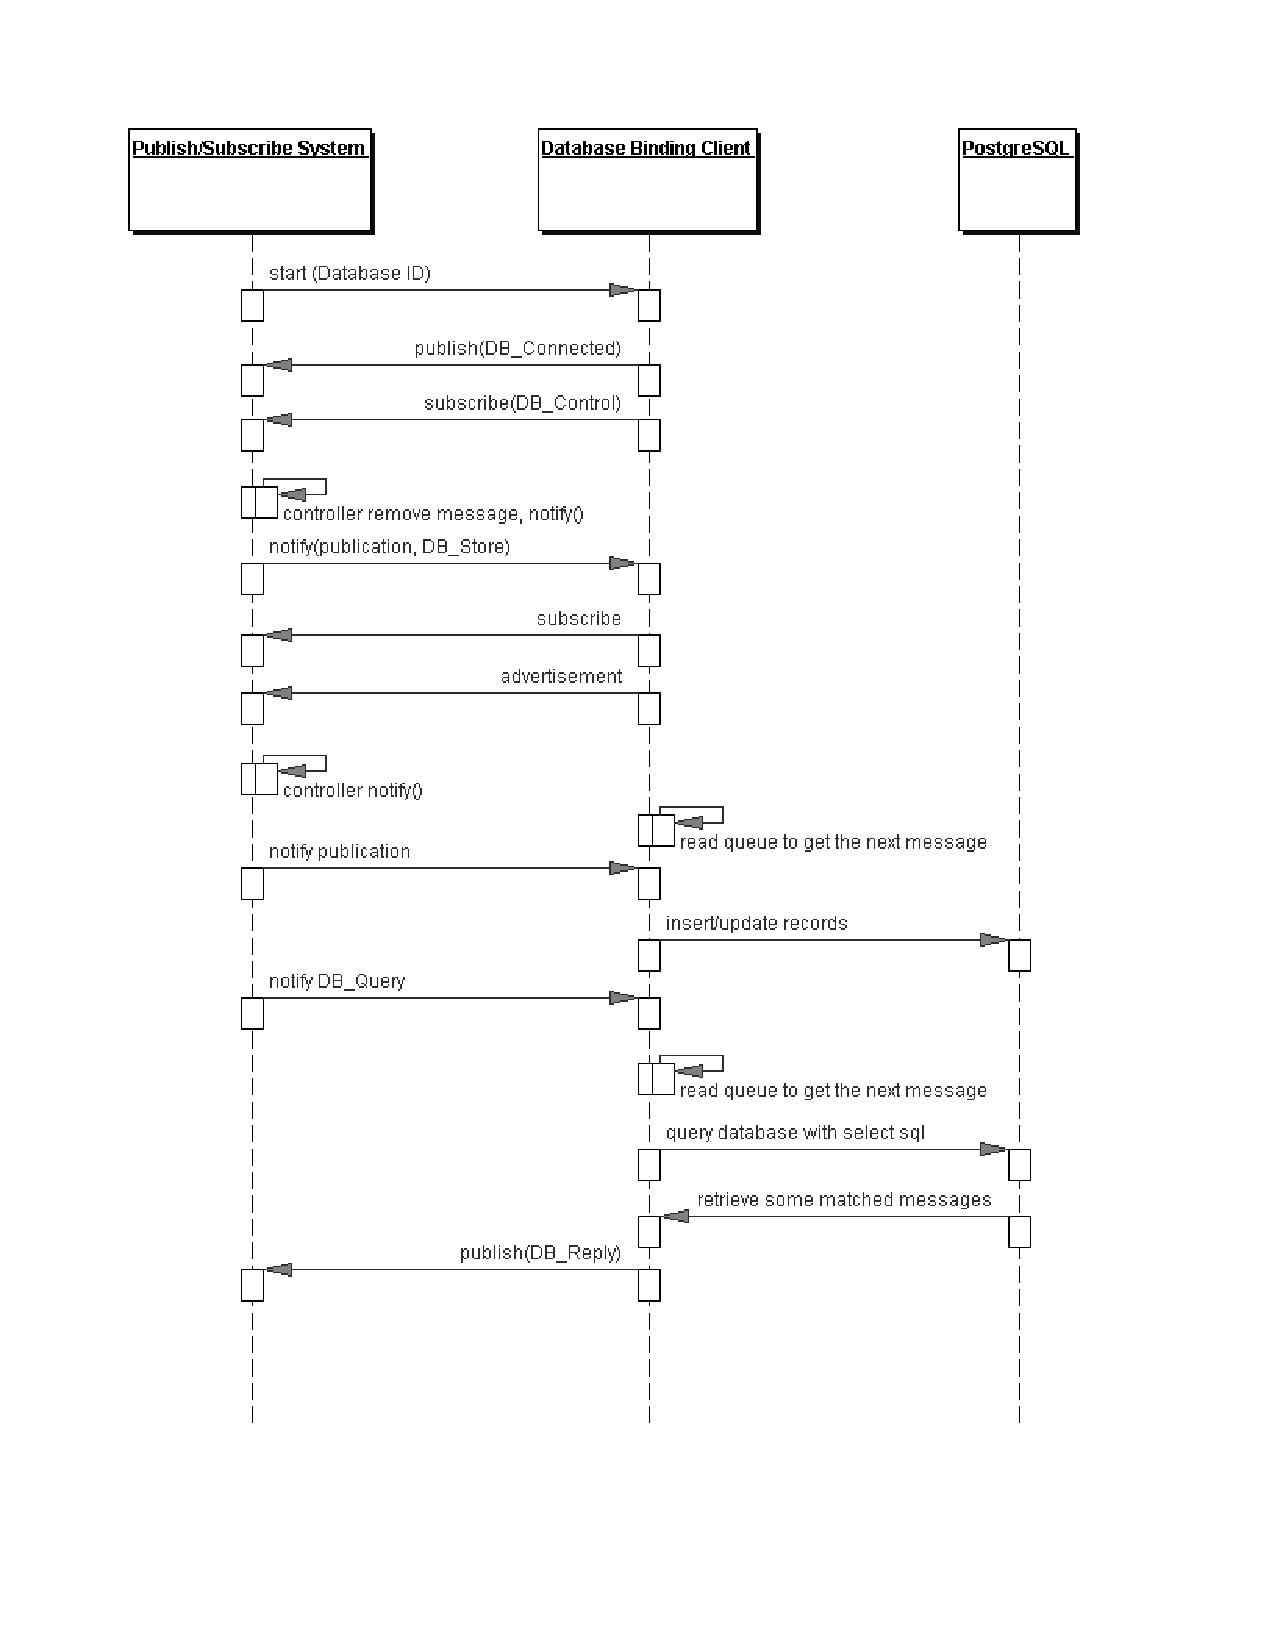
\includegraphics{dbbinding_seq}
\end{center}
\end{figure}

\subsection{Test Plan}    %The sixth part
\begin{itemize}
\item For database subscribe: insert events, historical queries on stored events into database.
\item For historical query: database receive \verb+db_query+, perform the look up in the database to get the relevant messages, publish \verb+db_reply+.
\item For database control: change publication to subscribe the appropriate message and advertise the same thing.
\end{itemize} 


\end{document}
